\documentclass[12pt]{report}
\usepackage{titlesec}
\usepackage{indentfirst}
\usepackage{hyperref}
\usepackage{hyphenat}
\usepackage{graphicx}
\usepackage{subcaption}
\usepackage{tocloft}

% pentru inserare de cod
\usepackage{listings}
\usepackage{color}

\definecolor{dkgreen}{rgb}{0,0.6,0}
\definecolor{gray}{rgb}{0.5,0.5,0.5}
\definecolor{mauve}{rgb}{0.58,0,0.82}

\lstset{frame=tb,
  language=C++,
  aboveskip=3mm,
  belowskip=3mm,
  showstringspaces=false,
  columns=flexible,
  basicstyle={\scriptsize\ttfamily},
  numbers=none,
  numberstyle=\tiny\color{gray},
  keywordstyle=\color{blue},
  commentstyle=\color{dkgreen},
  stringstyle=\color{mauve},
  breaklines=true,
  breakatwhitespace=true,
  tabsize=3
}
\renewcommand{\lstlistingname}{Sursa}

\graphicspath{ {Screenshots/} }

% for chapter dots in TOC
\renewcommand{\cftchapleader}{\cftdotfill{\cftdotsep}}
% rename bibliography
\renewcommand\bibname{Bibliografie}
% rename figure captions
\renewcommand{\figurename}{Figura}
% remove chapter numbering in document
\titleformat{\chapter}
  {\Large\bfseries} % format
  {}                % label
  {0pt}             % sep
  {\huge}           % before-code


\begin{document}

\begin{titlepage}
	\begin{center}
		\Large
		Colegiul Național Zinca Golescu, Pitești\\
		\vspace*{2cm}

		\Huge
		\textbf{Julia Set Explorer}

		\vspace{0.5cm}
		\LARGE
		Interactive fractal vizualizer

		\vspace{1.5cm}

		\textbf{Cioc Alex-Andrei}

		\vfill

		Lucrare de specialitate pentru examenul de atestare a competențelor profesionale

		\vspace{1.8cm}
		\Large
		Profilul Matematică--Informatică intensiv\\
		Profesor coordonator: Oprea Adriana\\
		Mai, 2020

	\end{center}
\end{titlepage}


\renewcommand*\contentsname{Cuprins}
\tableofcontents

\chapter{Prezentare generală}
Aplicația dezvoltă o temă interesantă, ce a căpătat un mare interes în ultimele decenii,
datorită dezvoltării graficii generate pe calculator. Încă cu câteva secole în urmă, matematicianul și filozoful
Gottfried Leibniz a considerat conceptul de autosimilaritate recursivă, aplicându-l pentru linii geometrice.
Probabil primele mulțimi de tip fractal au fost mulțimile lui Cantor, care aveau proprietăți matematice neobișnuite.
Însă, matematicienii erau limitați la ceea ce puteau vizualiza prin desenele manuale, ei neputând decât să ghicească formele spectaculoase pe care le creează aceste obiecte matematice.

Interesul pentru acest domeniu în epoca modernă îi poate fi datorat, într-o anumită măsură, lui Benoit Mandelbrot,
care a introdus termenul de ``fractal" și a arătat publicului, prin imagini generate de calculator,
frumusețea fractalilor. El a studiat orbitele numerelor complexe, atunci când se iterează după o anumită funcție, și
a definit mulțimea care acum îi poartă numele, ca fiind mulțimea tuturor punctelor a căror orbită este stabilă.
Având acces la calculatoare puternice, a ajuns să vadă pentru prima oară, în 1980, o imagine a fractalului său, lucru care l-a fascinat.
Astfel, a reușit să vizualizeze ceea ce se cheamă autosimilaritate, observând faptul că fractalul are o structură bine definită la scară oricât de mică.

Proiectul de față își propune să promoveze acest concept matematic, utilizând puterea de procesare a plăcilor grafice moderne, astfel, ilustrându-i frumusețea prin figuri plăcute ochiului.
De asemenea, se pot studia unele proprietăți interesante care leagă două mulțimi de tip fractal, Julia și Mandelbrot.

\begin{figure}
	\centering
	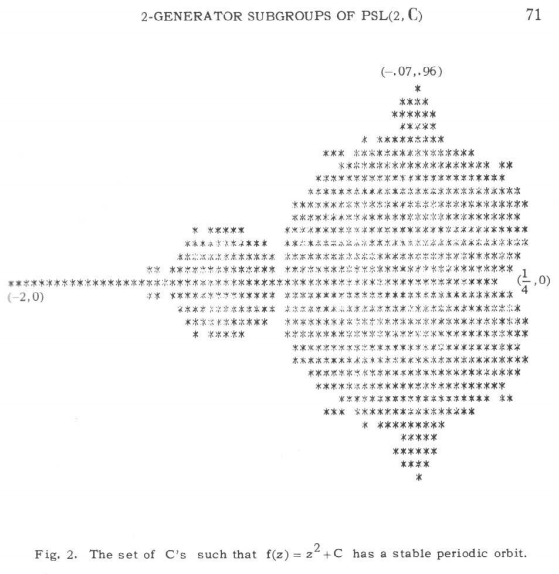
\includegraphics[scale=0.65]{Images/mandelbrot.png}
	\caption{Prima imagine a mulțimii Mandelbrot}
\end{figure}

\chapter{Cerințe de rulare}

Aplicația necesită Windows 10 pe arhitectura x64, precum și ultimul pachet de redistribuire Visual C++ pentru Visual Studio 2019 (tot pe x64).
Procesorul nu reprezintă un factor de limitare a performanței aplicației, însă trebuie, de asemenea, să suporte setul de instrucțiuni pe 64 de biți.
Placa video este recomandată a fi dedicată, și necesită suport pentru OpenGL 4.0, ea fiind utilizată la maxim în timpul rulării aplicației. Pentru modul UBER,
o placă video modernă ar fi de dorit.

În afară de pachetul care trebuie instalat, aplicația în sine ocupă mai puțin de 2 MB de memorie și alocă aproximativ 30 MB de memorie RAM și 40 MB VRAM în timpul execuției.

Testat pe un sistem cu CPU i5 6600, GPU RTX 2060 SUPER si 8 GB memorie RAM DDR4, aplicația redă minimum 900 FPS în modul normal,
respectiv minimum 200 FPS în modul UBER.

\chapter{Descrierea aplicației}

Aplicația este de tip executabil și creează o fereastră Fullscreen, în care va fi desenat fractalul.
Acesta se updatează în timp real după un parametru complex, care poate fi modificat cu ajutorul mouse-ului (click stânga),
și apare ca element grafic ca un punct roșu.

La deschiderea aplicației, se generează un parametru, aleator, din spațiul de ecran. De asemenea, se pot selecta, cu ajutorul tastelor numerice de la 0 la 9,
anumiți parametri prestabiliți, care generează figuri interesante, precum cea de mai jos
\begin{figure}[h]
	\centering
	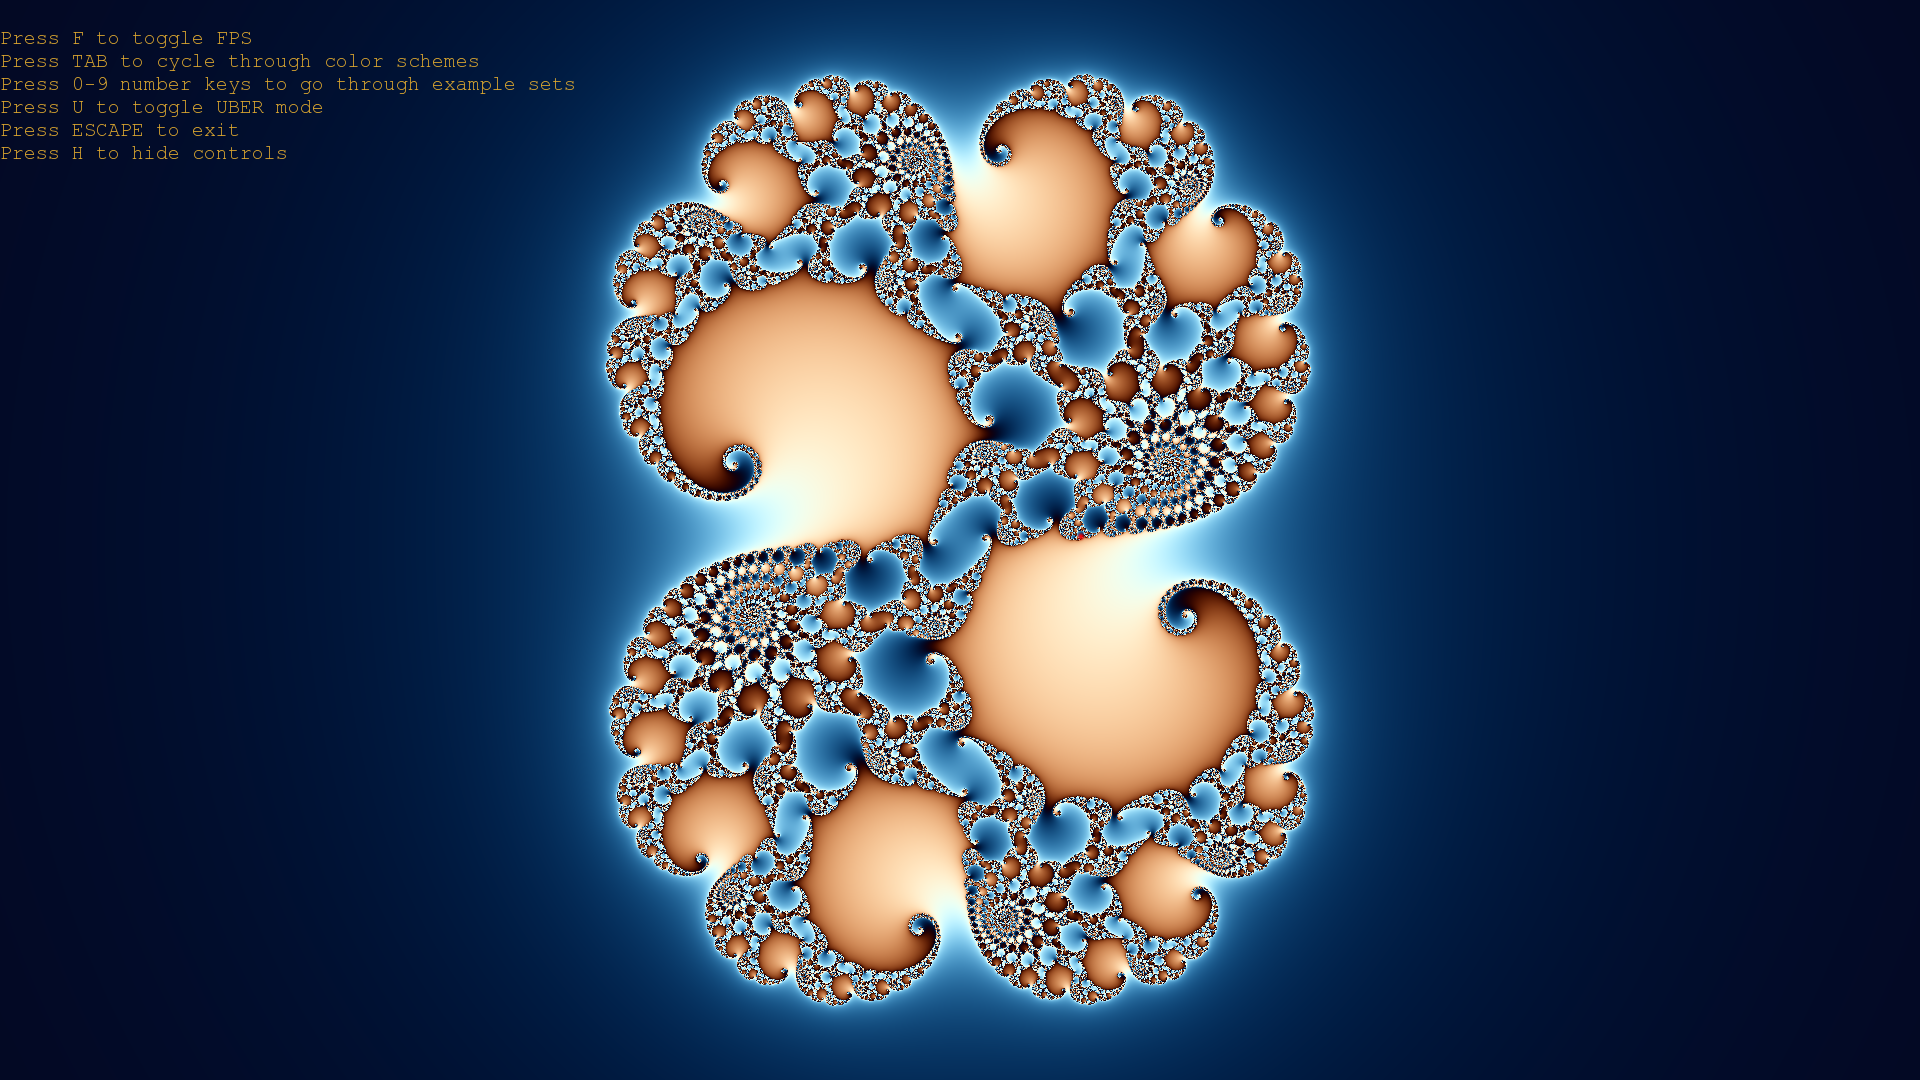
\includegraphics[width=\textwidth]{Images/example1.png}
	\caption{Mulțimea Julia pentru parametrul complex 0.28 + 0.008i}
\end{figure}
\\

Programul acceptă input de la tastatură, acesta fiind documentat în colțul din stânga sus
\begin{itemize}
	\item Tasta F afișează/ascunde contorul de FPS
	\item Tasta TAB schimbă modul de colorare a fractalului (sunt disponibile 4 moduri diferite, ca în imaginile de mai jos)
	      \begin{figure}[h]
		      \centering
		      \begin{subfigure}{.5\textwidth}
			      \centering
			      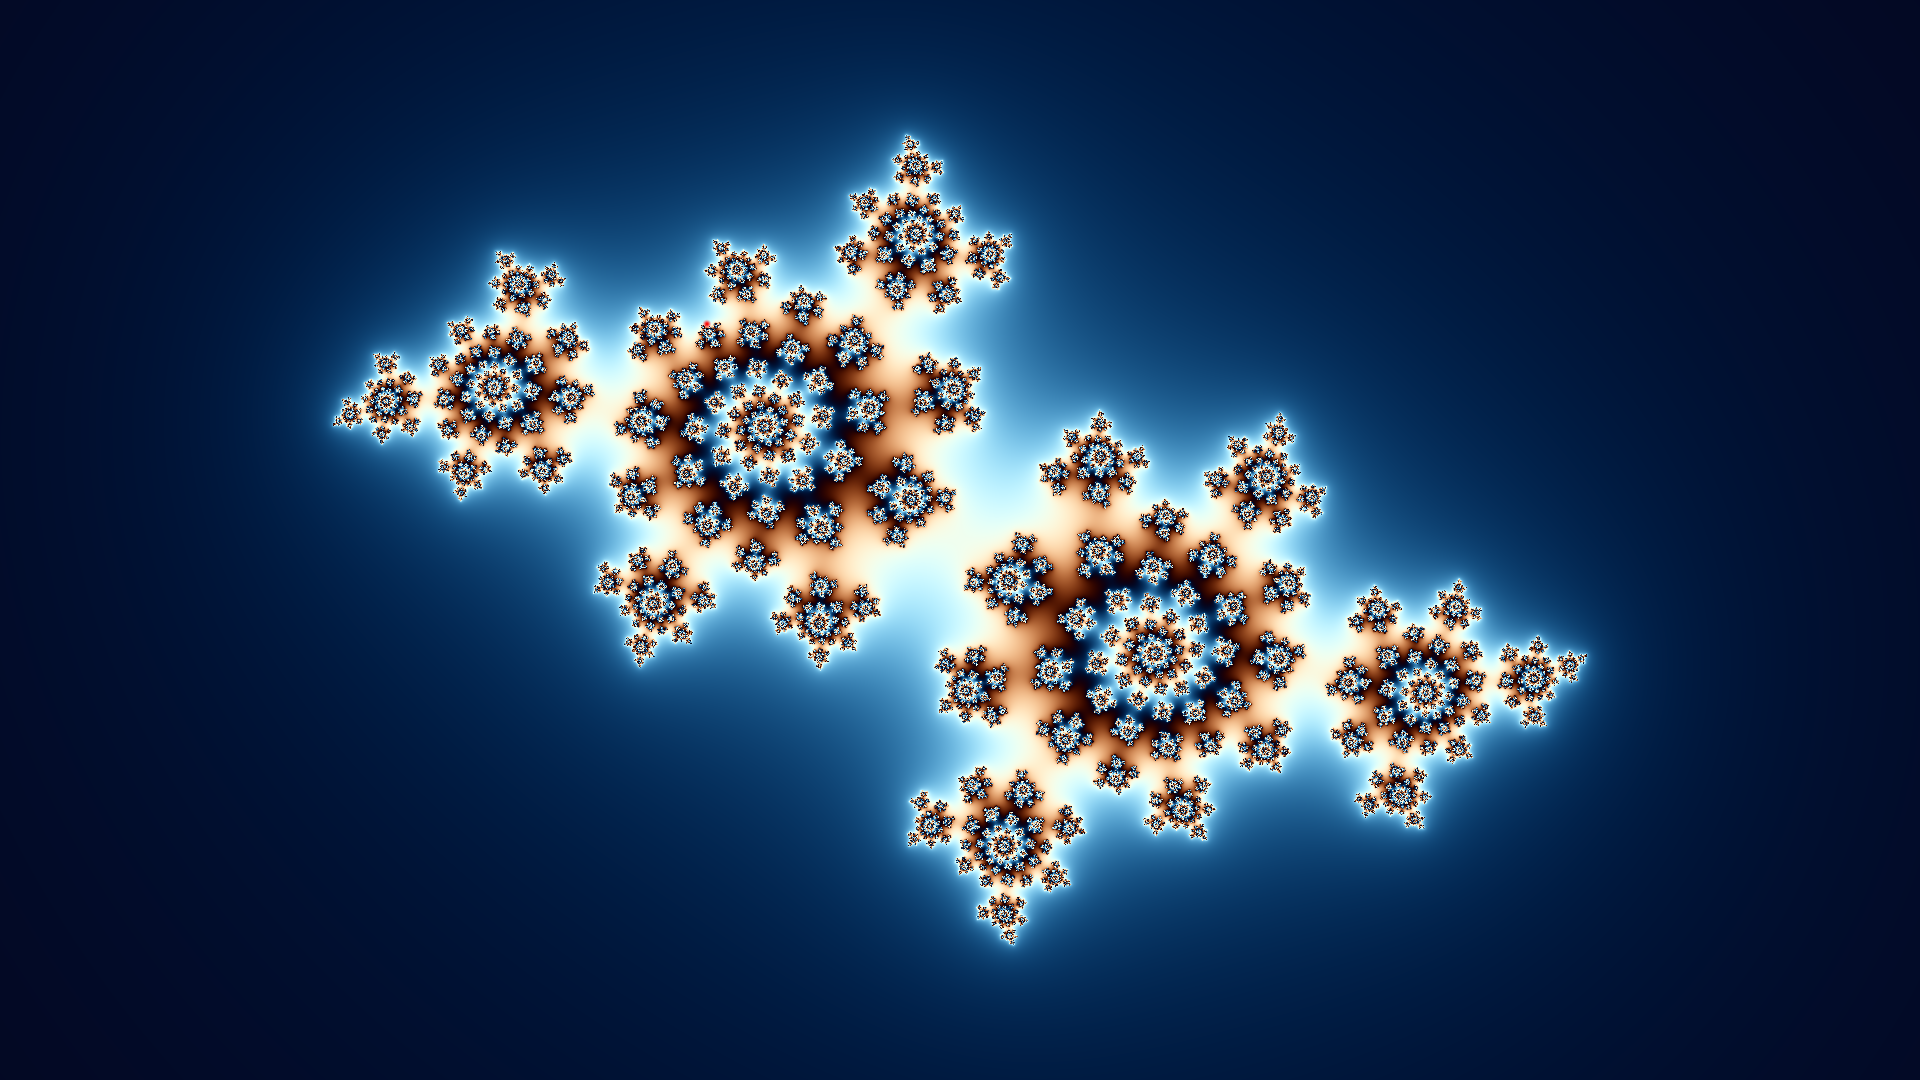
\includegraphics[width=0.8\textwidth]{Images/color1.png}
			      \caption{Modul default}
		      \end{subfigure}%
		      \begin{subfigure}{.5\textwidth}
			      \centering
			      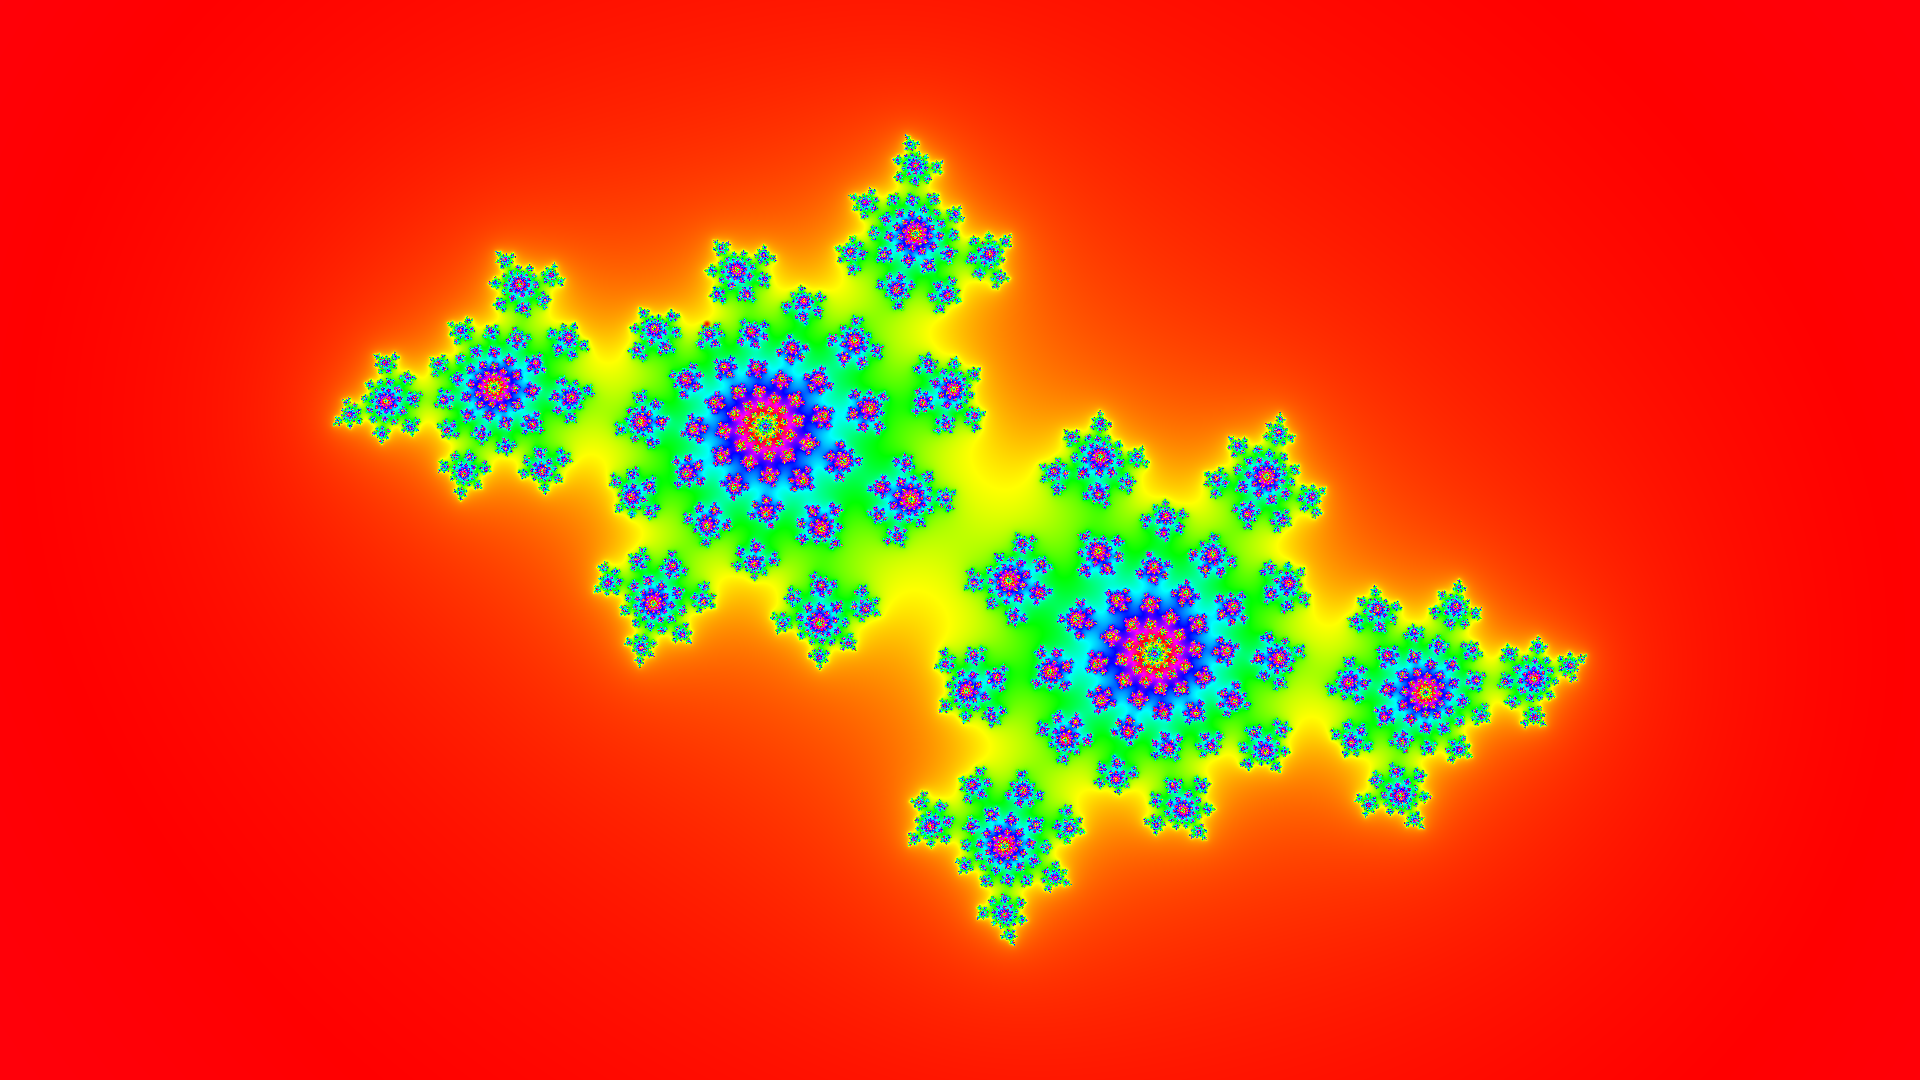
\includegraphics[width=0.8\textwidth]{Images/color2.png}
			      \caption{Modul multicolor}
		      \end{subfigure}
		      \begin{subfigure}{.5\textwidth}
			      \centering
			      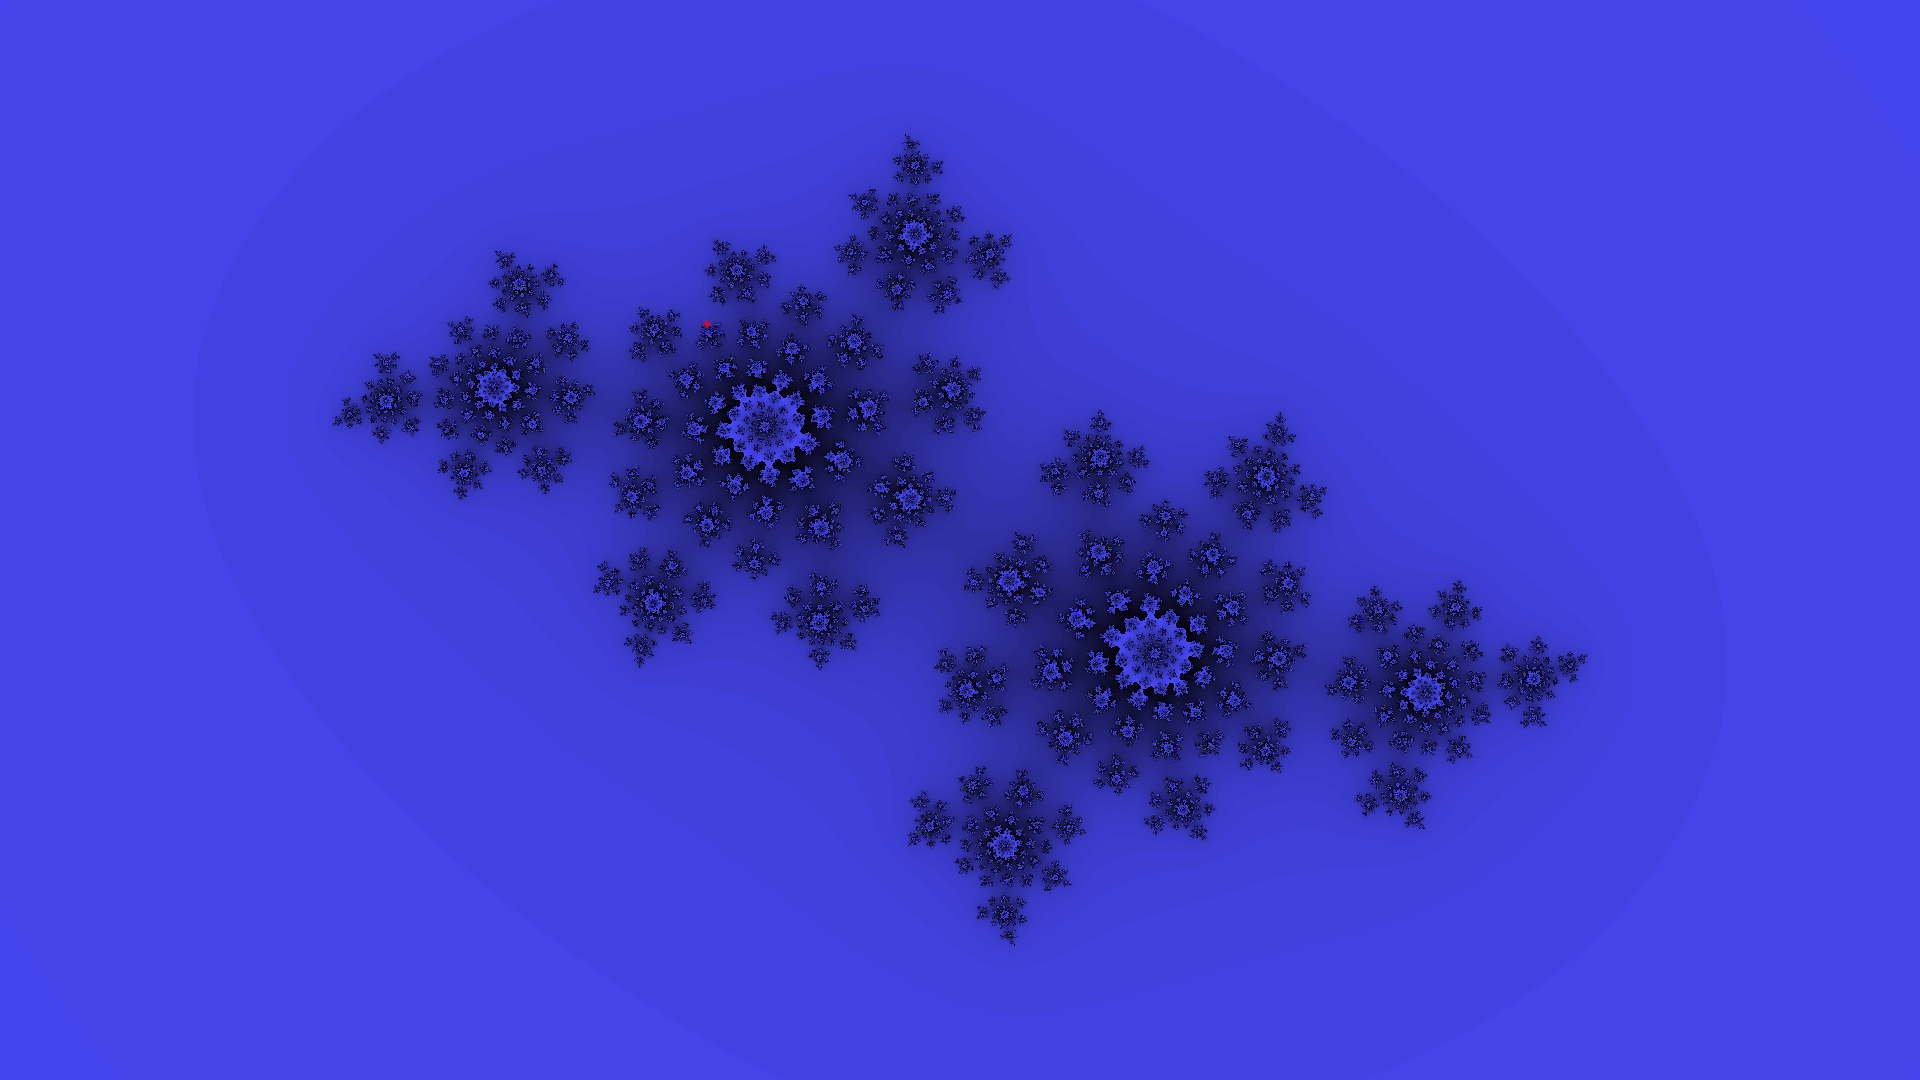
\includegraphics[width=0.8\textwidth]{Images/color3.png}
			      \caption{Modul bazat pe\\ numărarea iterațiilor}
		      \end{subfigure}%
		      \begin{subfigure}{.5\textwidth}
			      \centering
			      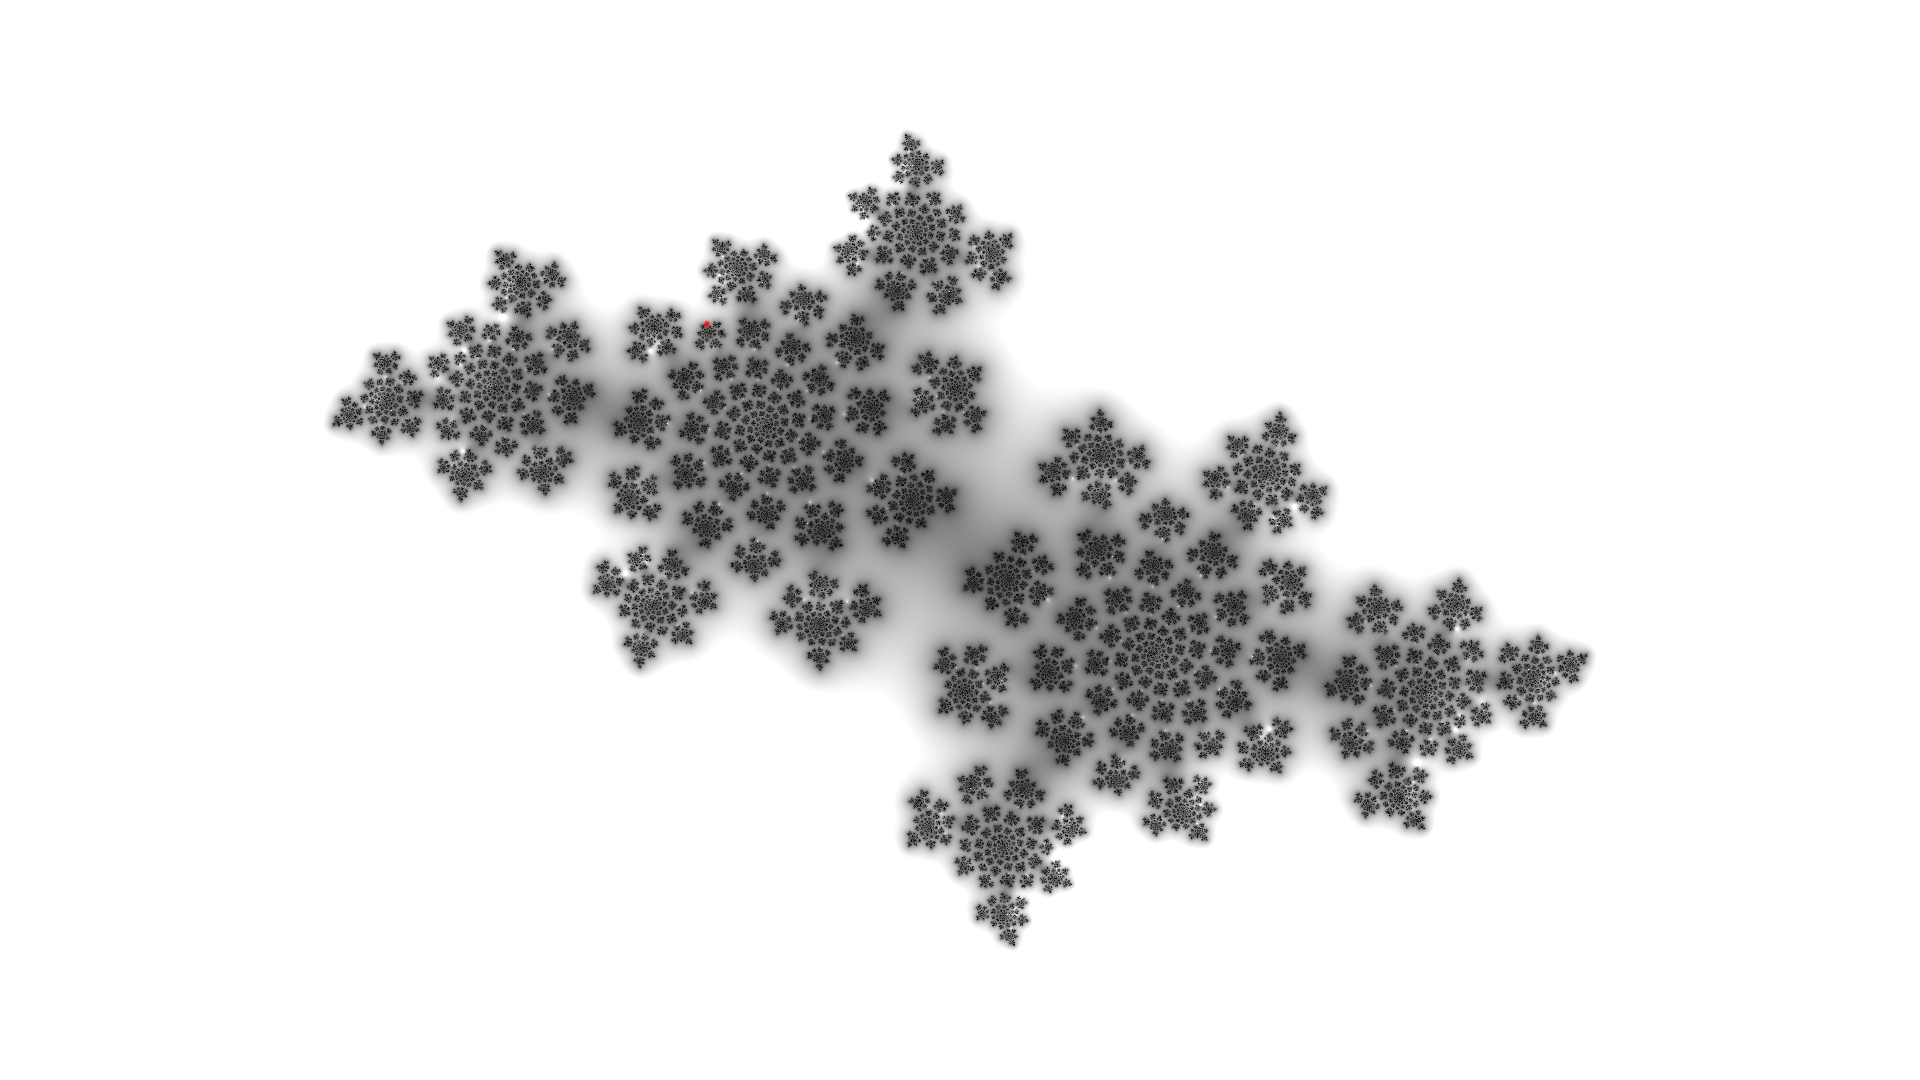
\includegraphics[width=0.8\textwidth]{Images/color4.png}
			      \caption{Modul bazat pe\\ estimarea distanței}
		      \end{subfigure}
	      \end{figure}
	      \\
	\item Tastele numerice 0-9 afișează anumite figuri prestabilite
	\item Tasta U activează modul UBER, care crește numărul de iterații desemnate aproximării fractalului,
	      ceea ce sporește acuratețea, dar scade drastic performanțele (este recomandat doar pentru plăci video mo\hyp{}derne)
	\item Tasta ESC închide aplicația
	\item Tasta H ascunde/afișează controalele.
\end{itemize}
Figura geometrică principală calculată este Mulțimea Julia ``umplută", gene\hyp{}rată prin iterarea funcției complexe
\(f(z) = z^2 + c\), unde \(z\) parcurge planul complex vizibil, pentru un parametru complex \(c\). Acest parametru este ori prestabilit, ori poate fi schimbat
prin click stânga pe ecran. În fragment shader, se normalizează coordonatele pixelilor pe ecran, de la spațiul rezoluției
la un spațiu care păstrează raportul de aspect și aduce valorile coordonatei \(y\) în intervalul \([-1,1]\). Astfel,
pixelul din mijlocul ecranului va avea coordonatele \((0,0)\). De asemenea, se aplică un zoom-out de magnitudine \(0,4\).

Mulțimea Julia pentru funcția \(f\) este definită ca fiind mulțimea tuturor numerelor complexe a căror orbită (parcursul pe care îl formează prin iterații repetate asupra funcției) se modifică drastic
la mici perturbări. Cu alte cuvinte, este frontiera mulțimii punctelor a căror orbită nu tinde către infinit.
Mulțimea Julia ``umplută" este reuniunea dintre mulțimea Julia și mulțimea formată din acele puncte care nu scapă spre infinit.

Pe ecran, vor apărea două tipuri de figuri Julia: unele care au un interior negru, bine definit, și altele care seamănă cu formațiuni discontinue.
Acestea sunt cele două tipuri de mulțimi Julia: conexe și neconexe. 

Proprietatea de conexitate este complet determinată de mulțimea Mandelbrot. Acesta este un alt fractal, strâns corelat cu Julia.
Este definit ca fiind mulțimea parametrilor complecși \(c\), pentru care orbita lui \(0\) obținută prin iterarea funcției
\(f(z) = z^2 + c\), nu tinde către infinit.
Mulțimea Julia asociată parametrului \(c\) este conexă dacă și numai dacă \(c\) aparține mulțimii Mandelbrot.
În caz negativ, aceasta este spațiu Cantor.

Aplicația afișează în fundal fractalul Mandelbrot, când butonul de click stânga este apăsat. Dacă punctul \(c\) aparține mulțimii Mandelbrot,
aceasta se colorează în verde, altfel, se colorează în roșu. Astfel, se evidențiază legătura dintre
cei doi fractali, un rezultat matematic remarcabil.

\chapter{Arhitectura aplicației}

Aplicația este scrisă în limbajul C++20, folosind interfața SFML 2.5.1 pentru grafică în OpenGL și gestionarea perifericelor de intrare.
Ca mediu de dezvoltare a fost folosit Visual Studio 2019, împreună cu compilatorul său integrat, MSVC.
Shaderele au fost scrise în GLSL. S-a folosit paradigma programării orientate pe obiecte.

Principalele clase sunt de tip singleton, \texttt{Game} și \texttt{Graphics}. În \texttt{Game} a fost programată logica aplicației, iar \texttt{Graphics} încapsulează
o fereastră de Windows, oferind metode de interfață pentru desenare.

Punctul de intrare al execuției este în fișierul \texttt{main.cpp}, unde se inițiali\hyp{}zează prin metoda \texttt{Setup} a clasei \texttt{Game}, apoi se ține firul de execuție într-o buclă în care se updatează starea aplicației cât timp este deschisă.
\begin{lstlisting}[caption=main.cpp]
// main.cpp
#include "Game.h"
#include "CustomExcept.h"

int main() {
	try {
		Game& game = Game::GetInstance();
		game.Setup();
		sf::RenderWindow& window = game.gfx.GetWindow();
		while( window.isOpen() ) {
			game.Go();
		}
	} catch( const CustomExcept & e ) {
		MessageBoxA( nullptr, e.what(), e.GetType(), MB_OK | MB_ICONEXCLAMATION );
	} catch( const std::exception & e ) {
		MessageBoxA( nullptr, e.what(), "Standard exception", MB_OK | MB_ICONEXCLAMATION );
	} catch( ... ) {
		MessageBoxA( nullptr, "Unknown exception.", "Unknown exception", MB_OK | MB_ICONEXCLAMATION );
	}

	return 0;
}
\end{lstlisting}

Blocul \texttt{try-catch} prinde excepțiile care sunt aruncate în timpul execuției, afișând într-o
fereastră detalii (căsuța este construită printr-un call către WinAPI). Clasa \texttt{CustomExcept}
este derivată din \texttt{std::exception} a librăriei standard și oferă informații suplimentare, precum fișierul și linia de cod care a aruncat excepția.
\begin{lstlisting}[caption = CustomExcept.h]
// CustomExcept.h
#pragma once
#include <exception>
#include <string>
#include <sstream>

// macro to insert the filename and the code line where the exception originated from
#define EXCEPT(s) (CustomExcept(__FILE__, __LINE__, s))

// custom exception class derived from the standard exception class
class CustomExcept : public std::exception {
public:
	CustomExcept() = delete;
	CustomExcept( const std::string& file, int line, const std::string& s );
	virtual const char* GetType() const;
	const char* what() const override;
private:
	mutable std::string buffer;
	std::string _file;
	int _line;
};
\end{lstlisting}
\begin{lstlisting}[caption = CustomExcept.cpp]
// CustomExcept.cpp
#include "CustomExcept.h"

CustomExcept::CustomExcept( const std::string& file, int line, const std::string& s )
	:
	buffer( s ),
	_line( line ),
	_file( file ) {}

const char* CustomExcept::GetType() const {
	return "Custom Exception";
}
// override function with custom message
const char* CustomExcept::what() const {
	std::ostringstream output;
	output << "[File]: " << _file << "\n[Line]: " << _line << "\n[Exception]: " << buffer;
	buffer = output.str();
	return buffer.c_str();
}
\end{lstlisting}

\newpage
Clasa \texttt{FrameTimer} este folosită pentru determinarea FPS-ului, și are drept metodă publică \texttt{Mark},
prin care se marchează timpul curent și se returnează timpul scurs de la ultima marcare.
\begin{lstlisting}[caption = FrameTimer.h]
// FrameTimer.h
#pragma once
#include <chrono>

// custom class to measure frame times
class FrameTimer {
public:
	FrameTimer();
	float Mark();
private:
	std::chrono::steady_clock::time_point last;
};
\end{lstlisting}
\begin{lstlisting}[caption = FrameTimer.cpp]
// FrameTimer.cpp
#include "FrameTimer.h"

using namespace std::chrono;

FrameTimer::FrameTimer() {
	last = steady_clock::now();
}
// mark the time in last and return the time passed since the last mark
float FrameTimer::Mark() {
	const auto old = last;
	last = steady_clock::now();
	const duration<float> frameTime = last - old;
	return frameTime.count();
}	
\end{lstlisting}

Clasa \texttt{SpriteObj} desemnează un obiect de tip sprite, care deține o ima\hyp{}gine, cu o anumită poziție pe ecran. Acesta poate fi desenat în framebuffer,
apelând metoda publică \texttt{Draw}.
\begin{lstlisting}[caption = SpriteObj.h]
// SpriteObj.h
#pragma once
#include <SFML/Graphics.hpp>
#include "Graphics.h"

// class that encapsulates sf::Texture and sf::Sprite for ease of use
class SpriteObj {
public:
	SpriteObj() = default;
	SpriteObj( const std::string& filename, const sf::Vector2f& pos = sf::Vector2f( 0.0f, 0.0f ), const sf::Vector2f& scale = sf::Vector2f( 1.0f, 1.0f ) );
	SpriteObj& operator=( const SpriteObj& other );

	void Draw( Graphics& gfx ) const;
	void CreateTexture( const sf::Vector2i& size );
	void CreateCanvas();
	sf::Vector2f GetPos() const noexcept;
	sf::Texture GetTexture() const noexcept;
	void SetTexture( const sf::Texture& texture );
	sf::Sprite GetSprite() const noexcept;
	void MoveTo( const sf::Vector2f& pos );
protected:
	sf::Vector2f _pos;
	sf::Texture _texture;
	sf::Sprite _sprite;
};
\end{lstlisting}
\begin{lstlisting}[caption = SpriteObj.cpp]
// SpriteObj.cpp
#include "SpriteObj.h"

SpriteObj::SpriteObj( const std::string& filename, const sf::Vector2f& pos, const sf::Vector2f& scale ) {
	_pos = pos;
	if( !_texture.loadFromFile( filename ) )
		throw EXCEPT( "Cannot load file: " + filename );
	_sprite.setTexture( _texture );
	_sprite.setScale( scale );
	_sprite.move( _pos );
}
SpriteObj& SpriteObj::operator=( const SpriteObj& other ) {
	if( this != &other ) {
		_pos = other._pos;
		_texture = other._texture;
		_sprite = other._sprite;
		_sprite.setTexture( _texture );
	}
	return *this;
}
// draw sprite to gfx window
void SpriteObj::Draw( Graphics& gfx ) const {
	gfx.Draw( GetSprite() );
}
// creates a blank texture of dimension size
void SpriteObj::CreateTexture( const sf::Vector2i& size ) {
	_texture.create( size.x, size.y );
	// update the sprite texture
	_sprite.setTexture( _texture );
}
// creates a texture that spans the whole window
void SpriteObj::CreateCanvas() {
	_texture.create( sf::VideoMode::getDesktopMode().width, sf::VideoMode::getDesktopMode().height );
	// update the sprite texture
	_sprite.setTexture( _texture );
}
sf::Vector2f SpriteObj::GetPos() const noexcept {
	return _pos;
}
sf::Texture SpriteObj::GetTexture() const noexcept {
	return _texture;
}
void SpriteObj::SetTexture( const sf::Texture& texture ) {
	_texture = texture;
	// update the sprite texture
	_sprite.setTexture( texture );
}
sf::Sprite SpriteObj::GetSprite() const noexcept {
	return _sprite;
}
void SpriteObj::MoveTo( const sf::Vector2f& pos ) {
	_sprite.move( pos - _pos );
	// set the position too
	_pos = pos;
}	
\end{lstlisting}

Clasa \texttt{Graphics} operează cu un singur membru, privat, care definește un tip de dată din SFML,
ce desemnează o fereastră utilizată pentru desenare. Conține o metodă, \texttt{Setup}, pentru inițializarea ferestrei cu numele \emph{Julia Explorer},
o iconiță customizată și extindere fullscreen, lucruri realizate cu ajutorul interfeței oferite de obiectul \texttt{window}.
Funcția \texttt{BeginFrame} golește framebufferul, în timp ce \texttt{EndFrame} îl afișează pe ecran.
\begin{lstlisting}[caption = Graphics.h]
// Graphics.h
#pragma once
#include <SFML/Graphics.hpp>
#include <Windows.h>
#include "CustomExcept.h"

// encapsulates a sf::RenderWindow object
class Graphics {
private:
	// constructor is private to prevent instantiation from outside
	Graphics() = default;
public:
	// singleton
	static Graphics& GetInstance() noexcept;
	Graphics( const Graphics& ) = delete;
	Graphics& operator=( const Graphics& ) = delete;
	Graphics( Graphics&& ) = delete;
	Graphics& operator=( Graphics&& ) = delete;

	sf::RenderWindow& GetWindow() noexcept;
	void Setup();
	void BeginFrame();
	void EndFrame();
	void Draw( const sf::Drawable& drawable, const sf::RenderStates& states = sf::RenderStates::Default );
	bool IsInWindow( const sf::Vector2f& pos ) const;
private:
	sf::RenderWindow window;
};
\end{lstlisting}
\begin{lstlisting}[caption = Graphics.cpp]
// Graphics.cpp	
#include "Graphics.h"
#include "CustomExcept.h"

Graphics& Graphics::GetInstance() noexcept {
	static Graphics _instance;
	return _instance;
}

sf::RenderWindow& Graphics::GetWindow() noexcept {
	return window;
}
// creates window
void Graphics::Setup() {
	window.create( sf::VideoMode::getDesktopMode(), "Julia Explorer", sf::Style::None );
	sf::Image icon;
	if( !icon.loadFromFile( "Content/Icon.png" ) )
		throw EXCEPT( "Cannot load file: Content/Icon.png" );
	window.setIcon( 16, 16, icon.getPixelsPtr() );
}
// stuff to do before drawing to the buffer
void Graphics::BeginFrame() {
	window.clear();
}
// stuff to do after drawing to the buffer
void Graphics::EndFrame() {
	window.display();
}
// function that takes an object that can be drawn and some state (e.g. shader) to apply, and draws it
void Graphics::Draw( const sf::Drawable& drawable, const sf::RenderStates& states ) {
	window.draw( drawable, states );
}

bool Graphics::IsInWindow( const sf::Vector2f& pos ) const {
	return (pos.x >= 0 && pos.x <= window.getSize().x - 1 && pos.y >= 0 && pos.y <= window.getSize().y - 1);
}	
\end{lstlisting}

Clasa \texttt{Game} asigură funcționarea aplicației conform regulilor și a comenzilor utilizatorului.
Metoda \texttt{Setup} inițializează variabilele care determină starea aplicației, încarcă resursele în memorie și apelează
funcția de \texttt{Setup} a ferestrei \texttt{gfx}.

Metoda \texttt{Go} este apelată în bucla din \texttt{main}. Aici, are loc începerea cadrului curent,
și se apelează metodele \texttt{UpdateModel} și \texttt{ComposeFrame}.
în cea dintâi, se gestionează evenimentele luate din coada ferestrei, inclusiv input de la mouse și tastatură.
De asemenea, se setează variabilele de tip \texttt{uniform} din shadere.
Funcția \texttt{ComposeFrame} desenează în buffer toate elementele vizibile pe ecran. La terminarea cadrului,
se apelează metoda \texttt{EndFrame} a obiectului \texttt{gfx} și se înregistrează frametime pentru FPS.
\begin{lstlisting}[caption = Game.h]
// Game.h
#pragma once
#include "Button.h"
#include "Graphics.h"
#include "FrameTimer.h"

class Game {
private:
	// constructor is private to prevent instantiation from outside
	Game() = default;
public:
	// singleton
	static Game& GetInstance() noexcept;
	Game( const Game& ) = delete;
	Game& operator=( const Game& ) = delete;
	Game( Game&& ) = delete;
	Game& operator=( Game&& ) = delete;

	void Setup();
	void ComposeFrame();
	void UpdateModel();
	void Go();
public:
	static Graphics& gfx;
private:
	SpriteObj canvas;
	sf::Shader fractalShader;
	bool hasFocus;		// focus of the window
	bool showFPS;
	bool showControls;
	bool uberMode;		// 4 times more iterations for more depth
	FrameTimer frameTimer;
	float updateTime;	// update rate for fps
	sf::Font textFont;
	sf::Text textFPS, textTAB;
	int colorScheme;	// varies from 0 to 3
	sf::Vector2f cPoints[10] = { {-0.1f, 0.651f}, {-1.0f, 0.0f}, {0.687f, 0.312f}, {0.295f, 0.55f}, {-0.4f, 0.6f}, {0.25f, 0.0f}, {0.28f, 0.008f}, {-0.12f,-0.77f}, {-0.79f,0.15f}, {0.0f, -0.8f} };	// examples of julia sets
};
\end{lstlisting}
\newpage
\begin{lstlisting}[caption = Game.cpp]
// Game.cpp	
#include "Game.h"
#include <algorithm>
#include <string>
#include <conio.h>
#include <cmath>
#include <random>

Graphics& Game::gfx = Graphics::GetInstance();

Game& Game::GetInstance() noexcept {
	static Game _instance;
	return _instance;
}
// setup graphics and load things
void Game::Setup() {
	// load shader
	if( !sf::Shader::isAvailable )
		throw EXCEPT( "Shaders are not available on this system" );
	if( !fractalShader.loadFromFile( "Shaders/vertex.vert", "Shaders/fractal.frag" ) )
		throw EXCEPT( "Cannot load shaders" );
	// set resolution uniform
	fractalShader.setUniform( "Resolution", sf::Vector2f( sf::VideoMode::getDesktopMode().width, sf::VideoMode::getDesktopMode().height ) );
	// load text font
	if( !textFont.loadFromFile( "Content/cour.ttf" ) )
		throw EXCEPT( "Cannot load file: Content/cour.ttf" );
	textFPS.setFont( textFont );
	textTAB.setFont( textFont );
	textFPS.setFillColor( { 222, 168, 47 } );
	textTAB.setFillColor( { 222, 168, 47 } );
	textTAB.setPosition( { 0.0f, 24.0f } );
	textFPS.setCharacterSize( 20 );
	textTAB.setCharacterSize( 20 );
	textTAB.setString( "Press F to toggle FPS\nPress TAB to cycle through color schemes\nPress 0-9 number keys to go through example sets\nPress U to toggle UBER mode\nPress ESCAPE to exit\nPress H to hide controls" );
	// setup window
	canvas.CreateCanvas();
	gfx.Setup();
	// set random red dot position inside the window
	std::random_device dev;
	std::mt19937 rng( dev() );
	std::uniform_int_distribution<std::mt19937::result_type> randHeight( 0, gfx.GetWindow().getSize().y - 1 );
	std::uniform_int_distribution<std::mt19937::result_type> randWidth( 0, gfx.GetWindow().getSize().x - 1 );
	sf::Vector2f randomPoint = sf::Vector2f( randWidth( rng ), randHeight( rng ) );
	fractalShader.setUniform( "RedDotPos", randomPoint );
	fractalShader.setUniform( "IsExample", false );
	fractalShader.setUniform( "ColorScheme", 0 );
	// initialize member variables
	hasFocus = true;
	showFPS = false;
	showControls = true;
	uberMode = false;
	colorScheme = 0;	// default color scheme
}
// updates game logic
void Game::UpdateModel() {
	static auto& window = gfx.GetWindow();
	// event queue
	sf::Event event;
	while( window.pollEvent( event ) )
		switch( event.type ) {
			case sf::Event::Closed:
				window.close();
				return;
			case sf::Event::GainedFocus:
				hasFocus = true;
				break;
			case sf::Event::LostFocus:
				hasFocus = false;
				break;
			case sf::Event::KeyPressed:
				// exit
				if( hasFocus && event.key.code == sf::Keyboard::Escape ) {
					window.close();
					return;
				}
				// toggle FPS
				else
					if( event.key.code == sf::Keyboard::F ) {
						showFPS = showFPS ? false : true;
						updateTime = 0.25; // for resetting fps
					}
				// switch color scheme
					else
						if( event.key.code == sf::Keyboard::Tab ) {
							colorScheme = (colorScheme + 1) % 4;
							fractalShader.setUniform( "ColorScheme", colorScheme );
						}
				// toggle controls
						else
							if( event.key.code == sf::Keyboard::H )
								showControls = showControls ? false : true;
				// change example
							else
								if( event.key.code >= sf::Keyboard::Num0 && event.key.code <= sf::Keyboard::Num9 ) {
									fractalShader.setUniform( "RedDotPos", cPoints[event.key.code - sf::Keyboard::Num0] );
									fractalShader.setUniform( "IsExample", true );
								}
				// toggle UBER
								else
									if( event.key.code == sf::Keyboard::U ) {
										uberMode = uberMode ? false : true;
										fractalShader.setUniform( "UBER", uberMode );
									}
				break;
		}
	// step out if out of focus
	if( !hasFocus )
		return;

	// set the uniforms: update mouse position only if LMB is pressed
	if( sf::Mouse::isButtonPressed( sf::Mouse::Left ) && gfx.IsInWindow( sf::Vector2f( sf::Mouse::getPosition( gfx.GetWindow() ) ) ) ) {
		fractalShader.setUniform( "IsLMBPressed", true );
		fractalShader.setUniform( "RedDotPos", sf::Vector2f( sf::Mouse::getPosition( gfx.GetWindow() ) ) );
		fractalShader.setUniform( "IsExample", false );
	} else
		fractalShader.setUniform( "IsLMBPressed", false );
}
// draws the objects on the screen
void Game::ComposeFrame() {
	// draw the canvas and apply the shader
	gfx.Draw( canvas.GetSprite(), &fractalShader );
	// show FPS
	if( showFPS )
		gfx.Draw( textFPS );
	// show controls
	if( showControls )
		gfx.Draw( textTAB );
}
// main game loop
void Game::Go() {
	if( hasFocus )
		gfx.BeginFrame();

	// go through this even if out of focus, to handle the event queue
	UpdateModel();

	if( hasFocus ) {
		ComposeFrame();
		gfx.EndFrame();
	}

	// show FPS
	auto frameTime = frameTimer.Mark();
	if( showFPS ) {
		updateTime += frameTime;
		if( updateTime > 0.25 ) {
			updateTime -= 0.25;
			textFPS.setString( "FPS: " + std::to_string( int( 1.0 / frameTime ) ) );
		}
	}
}
\end{lstlisting}

\newpage
Aplicația utilizează un fragment shader și un vertex shader pentru desenarea accelerată a fractalilor cu ajutorul plăcii video.
Vertex shader se execută o dată la fiecare cadru, iar aici, în cazul în care ținem click stânga apăsat, calculăm dacă parametrul reprezentat de punctul roșu se află în mulțimea Mandelbrot,
pe care o vom colora (în fragment shader) verde, în caz afirmativ, respectiv roșu, altfel.

În fragment shader, care se execută pentru fiecare pixel de pe ecran, calculăm dacă pixelul curent
se află în interiorul definit de frontiera mulțimii Julia (acele puncte a căror orbită rămâne stabilă).
Pe acestea le colorăm în negru. Dacă este setat modul UBER, numărul de iterații pentru determinarea orbitei crește
de la 300 la 2000. În cazul în care mulțimea Julia nu este conectată, nu am putea desena niciun punct negru pe ecran, practic, pentru că
mulțimea ar căpăta, impropriu spus, formă de praf. De aceea, se folosesc metode de colorare, care aproximează distanța față de mulțime,
sau iau în calcul numărul de iterații necesare pentru ca orbita punctului să devină haotică.
\begin{lstlisting}[caption = vertex.vert]
	// vertex.vert	
	varying float rzMand;
	varying vec2 juliaParam;
	
	uniform vec2 Resolution;
	uniform vec2 RedDotPos;
	uniform bool IsExample;
	uniform bool IsLMBPressed;
	
	void main() {
		// transform the vertex position
		gl_Position = gl_ModelViewProjectionMatrix * gl_Vertex;
		// transform the texture coordinates
		gl_TexCoord[0] = gl_TextureMatrix[0] * gl_MultiTexCoord0;
		// forward the vertex color
		gl_FrontColor = gl_Color;
		
		float zoom = 0.4;
		// update redDot as mouse position or as example position
		if (!IsExample) {
			juliaParam = (RedDotPos - Resolution * 0.5) / Resolution.y;
			// invert the mouse y coordinates
			juliaParam.y = -juliaParam.y;
			juliaParam /= zoom;
		}
		else
		juliaParam = RedDotPos;
		
		// check if juliaParam is in mandelbrot set (check its orbit)
		// only when LMB is pressed
		if (IsLMBPressed) {
			vec2 z = vec2(0.0);
			rzMand = 0.0;
			vec2 c = juliaParam;
			for(int i = 0; i < 50; i ++ )
			{
				if (rzMand > 4.0)
				break;
				
				// Z -> Z^2 + c
				z = vec2(z.x * z.x - z.y * z.y, 2.0 * z.x * z.y) + c;
				rzMand = dot(z, z);
			}
		}
	}
	\end{lstlisting}
\begin{lstlisting}[caption = fragment.frag]
// fragment.frag
precision highp float;

uniform vec2 Resolution;
uniform vec2 RedDotPos;
uniform bool IsLMBPressed;
uniform bool IsExample;
uniform bool UBER;
uniform int ColorScheme;

varying float rzMand;
varying vec2 juliaParam;

// colors used to blend on one color scheme
const vec3 colorMix1 = vec3(0.2824, 0.2824, 0.9686);
const vec3 colorMix2 = vec3(0.0, 0.0, 0.0);

// hue-saturation-value to rgb conversion
vec3 hsv2rgb(float c)
{
    vec3 rgb = clamp(abs(mod(c * 6.0 + vec3(0.0, 4.0, 2.0), 6.0) - 3.0) - 1.0, 0.0, 1.0);
    return rgb;
}

void main()
{
    // normalize coordinates, such that y axis goes from -1 to 1, (0, 0) is the center of the screen, keep aspect ratio
    vec2 uv = (gl_FragCoord.xy - Resolution * 0.5) / Resolution.y;
    
    // set and apply zoom
    float zoom = 0.4;
    uv /= zoom;
    
    // Julia Set
    vec2 z = uv;
    vec2 c = juliaParam;
    vec2 dz = vec2(0.0);
    float rz = 0.0;
    float rdz = 0.0;
    int juliaIter = 300;
    
    if (UBER)
    juliaIter = 2000;
    
    // Julia Set iteration
    int i;
    for(i = 0; i < juliaIter; i ++ )
    {
        if (rz > 1024.0)
        break;
        
        if (ColorScheme == 3)
        // Z' -> 2*Z*Z' + 1
        dz = 2.0 * vec2(z.x * dz.x - z.y * dz.y, z.x * dz.y + z.y * dz.x) + vec2(1.0, 0.0);
        // Z -> Z^2 + c
        z = vec2(z.x * z.x - z.y * z.y, 2.0 * z.x * z.y) + c;
        rz = dot(z, z);
    }
    
    // (COLORING ALGORITHMS) https://www.mi.sanu.ac.rs/vismath/javier/b3.htm
    vec3 color;
    if (rz < 4.0)
    color = vec3(0.0);
    else {
        // normalized iteration count: https://iquilezles.org/www/articles/mset_smooth/mset_smooth.htm
        float nic = float(i) + 1.0 - log2(log2(rz));
        
        if (ColorScheme == 1)
        // multicolored
        color = (hsv2rgb(nic * 0.015));
        else if (ColorScheme == 2)
        // (discrete) escape time coloring: Base the color on the number of iterations
        color = mix(colorMix1, colorMix2, fract(float(i) * 0.02));
        else if (ColorScheme == 3) {
            // (DISTANCE ESTIMATOR) https://iquilezles.org/www/articles/distancefractals/distancefractals.htm
            rdz = dot(dz, dz);
            float distJulia = 0.5 * sqrt(rz / rdz) * log(rz);
            distJulia = clamp(pow(6.0 * distJulia / zoom, 0.2), 0.0, 1.0);
            // greyscale, distance estimation
            color = vec3(distJulia);
        }
        else
        // default color scheme, like on wikipedia
        color = 0.5 + 0.5 * cos(3.0 + nic * 0.2 + vec3(0.0, 0.6, 1.0));
    }
    
    // Mandelbrot Set (shown when left mouse button is pressed)
    if (IsLMBPressed) {
        // set the color of the Mandelbrot Set, according to the inclusion of the juliaParam in it
        vec3 incolor;
        if (rzMand < 4.0)
        incolor = vec3(0.3, 1.0, 0.3); // is in
        else if (ColorScheme == 1)// adjust red color for the multicolored one
        incolor = vec3(0.4, 0.0667, 0.0039); // is out
        else
        incolor = vec3(0.9059, 0.1843, 0.0588); // is out
        
        // draw the Mandelbrot Set
        z = vec2(0.0);
        rz = 0.0;
        c = uv;
        for(i = 0; i < 50; i ++ )
        {
            if (rz > 16.0)
            break;
            
            // Z -> Z^2 + c
            z = vec2(z.x * z.x - z.y * z.y, 2.0 * z.x * z.y) + c;
            rz = dot(z, z);
        }
        
        vec3 color2;
        if (rz < 4.0)
        color2 = incolor;
        else {
            float nic = float(i) + 1.0 - log2(log2(rz));
            color2 = mix(color, vec3(1.0), smoothstep(0.0, 60.0, nic));
        }
        
        color = mix(color, color2, 0.3);
    }
    
    // red dot
    color = mix(color, vec3(1.0, 0.0, 0.0), smoothstep(5.0 / zoom / Resolution.y, 0.0, length(uv - juliaParam)));
    
    gl_FragColor = vec4(color, 1.0);
}
\end{lstlisting}

\chapter{Extindere}
Aplicația poate fi extinsă prin adăugarea unui mod de playback automat a unor animații, prin schimbarea paletei de culori în timp real,
sau prin adăugarea de noi metode de colorare.

Pentru un nivel și mai avansat, ar putea accepta mai multe funcții care să genereze mulțimile Julia,
chiar să poată fi parsate de la tastatură, într-un format convenabil. O extindere în 3D, folosind cuaternioni,
ar fi și mai interesantă, datorită introducerii efectelor de iluminare.
\begin{figure}[h]
	\centering
	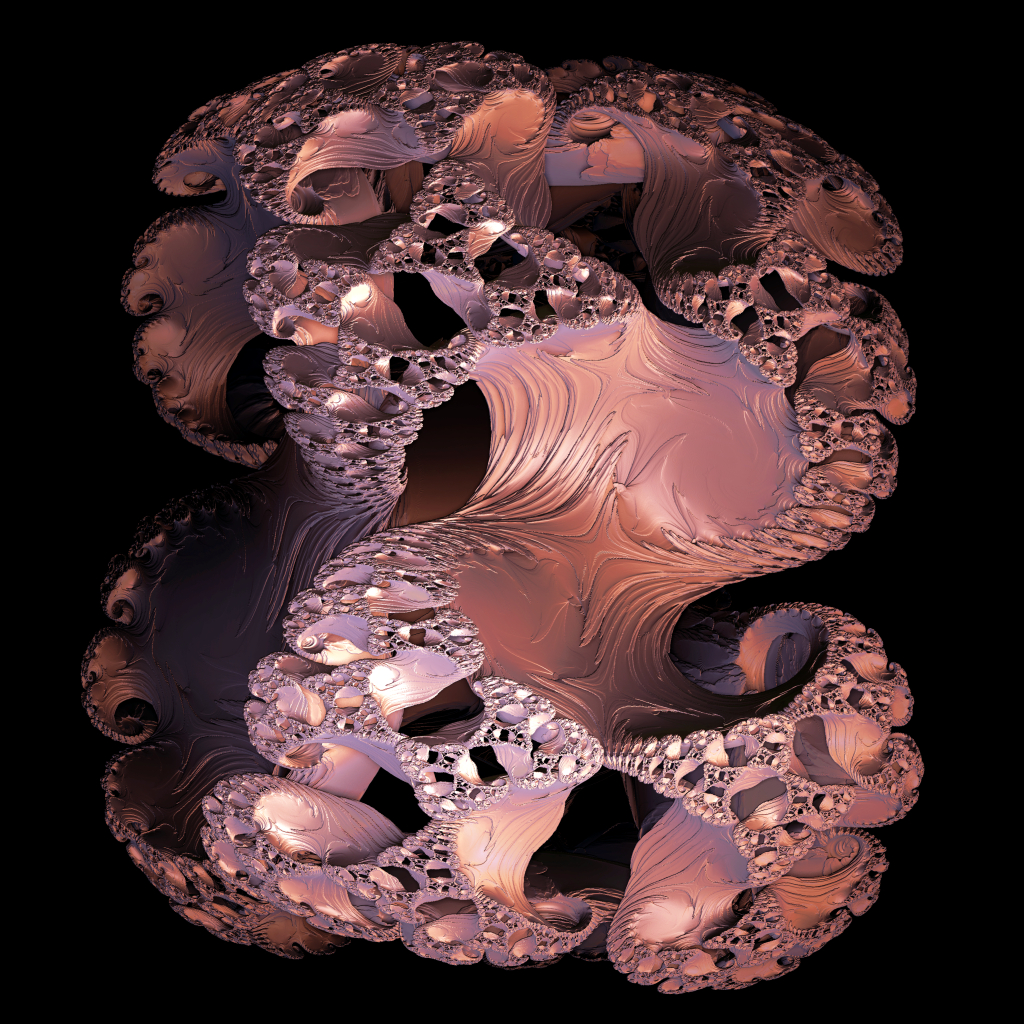
\includegraphics[width=.6\textwidth]{"Images/3DJulia.jpg"}
	\caption{Exemplu de randare 3D}
\end{figure}

\begin{thebibliography}{9}
	\bibitem{sfml}
	https://www.sfml-dev.org/
	\bibitem{iq}
	https://iquilezles.org/www/index.htm
	\bibitem{shadertoy}
	https://www.shadertoy.com/
	\bibitem{def}
	http://blog.hvidtfeldts.net/index.php/2011/06/distance-estimated-3d-fractals-part-i/
	\bibitem{cpp}
	https://en.cppreference.com/w/
	\bibitem{opengl}
	https://www.khronos.org/registry/OpenGL-Refpages/gl4/
\end{thebibliography}

\end{document}